\documentclass[a4paper,12pt]{article}
\usepackage{tkz-euclide}
\usepackage{gensymb}
\usepackage[utf8]{inputenc}
\usepackage{graphicx}
\title{ASSIGNMENT-5}
\author{SENANI SADHU}
\date{\today}
\begin{document}
	\maketitle
	\pagenumbering{roman}
	\section{Question:-}
	\paragraph{Construct right angled $\Delta$ whose hypotenuse is 6 and one of the legs is 4.}
	\section{Solution:-}
	Given,\\
	Hypotenuse=6 , Side=4\\
	Let the triangle be $\Delta$ABC with $\angle$B=90$^{\circ}$ AC=6,BC=4
	\subsection{Steps of Construction:-}
	\begin{itemize}
		\item Draw a line segement Bc of length a=4
		\item Now, we draw 90$^{\circ}$ from point B.
		\item Takine C as center,6cm as radius , we draw an arc.\\
		Let  the point  where arc intersects  the ray be point A.
		\item Join AC.
	\end{itemize}
\paragraph{$\Delta$ABC is required triangle.}
\subsection{Figure:-}
\subsubsection{Using Tikz-Latex:}
\begin{center}
	\begin{tikzpicture}
		\draw(0,0)--(4,0);
		\draw(0,0)--(90:8cm);
		\node at (0,0)[below left]{$B$};
		\node at (4,0)[below left]{$C$};
		\draw(-0.3,2.5) arc (150:120:2cm);
		\draw(-0.3,3.1) arc (60:30:2cm);
		\node at (0,8)[above left]{$X$};
		\draw(-0.3,4.47) arc (150:120:2cm);
		\draw(0,4.85)--(4,0);
		\node at (0,4.85)[above left]{$A$};
	\end{tikzpicture}
\end{center}
\subsubsection{Output of Python code:}
\begin{figure}[htp]
	\centering
	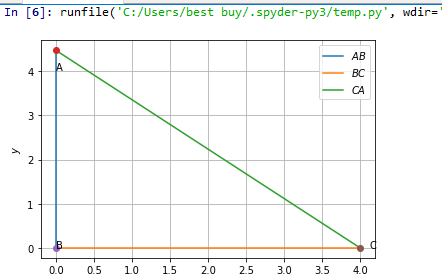
\includegraphics[width=10cm]{triangle.png}
	\caption{Fig generated using python}
\end{figure}
\end{document}